\documentclass[aspectratio=169]{beamer}


\usetheme{vega}
\renewcommand{\textSupervisors}    {Supervisor}

\title{Forecasting the Yield Curve: An Econometric Study}
\subtitle{}
\author{Vsevolod Zaostrovsky, Ivan Cherepakhin, Artemy Sazonov}
\institute{Lomonosov Moscow State University}
\supervisor{Ivan P. Stankevich}

\begin{document}
\maketitle

\begin{frame}{YC and data}
    \begin{figure}
        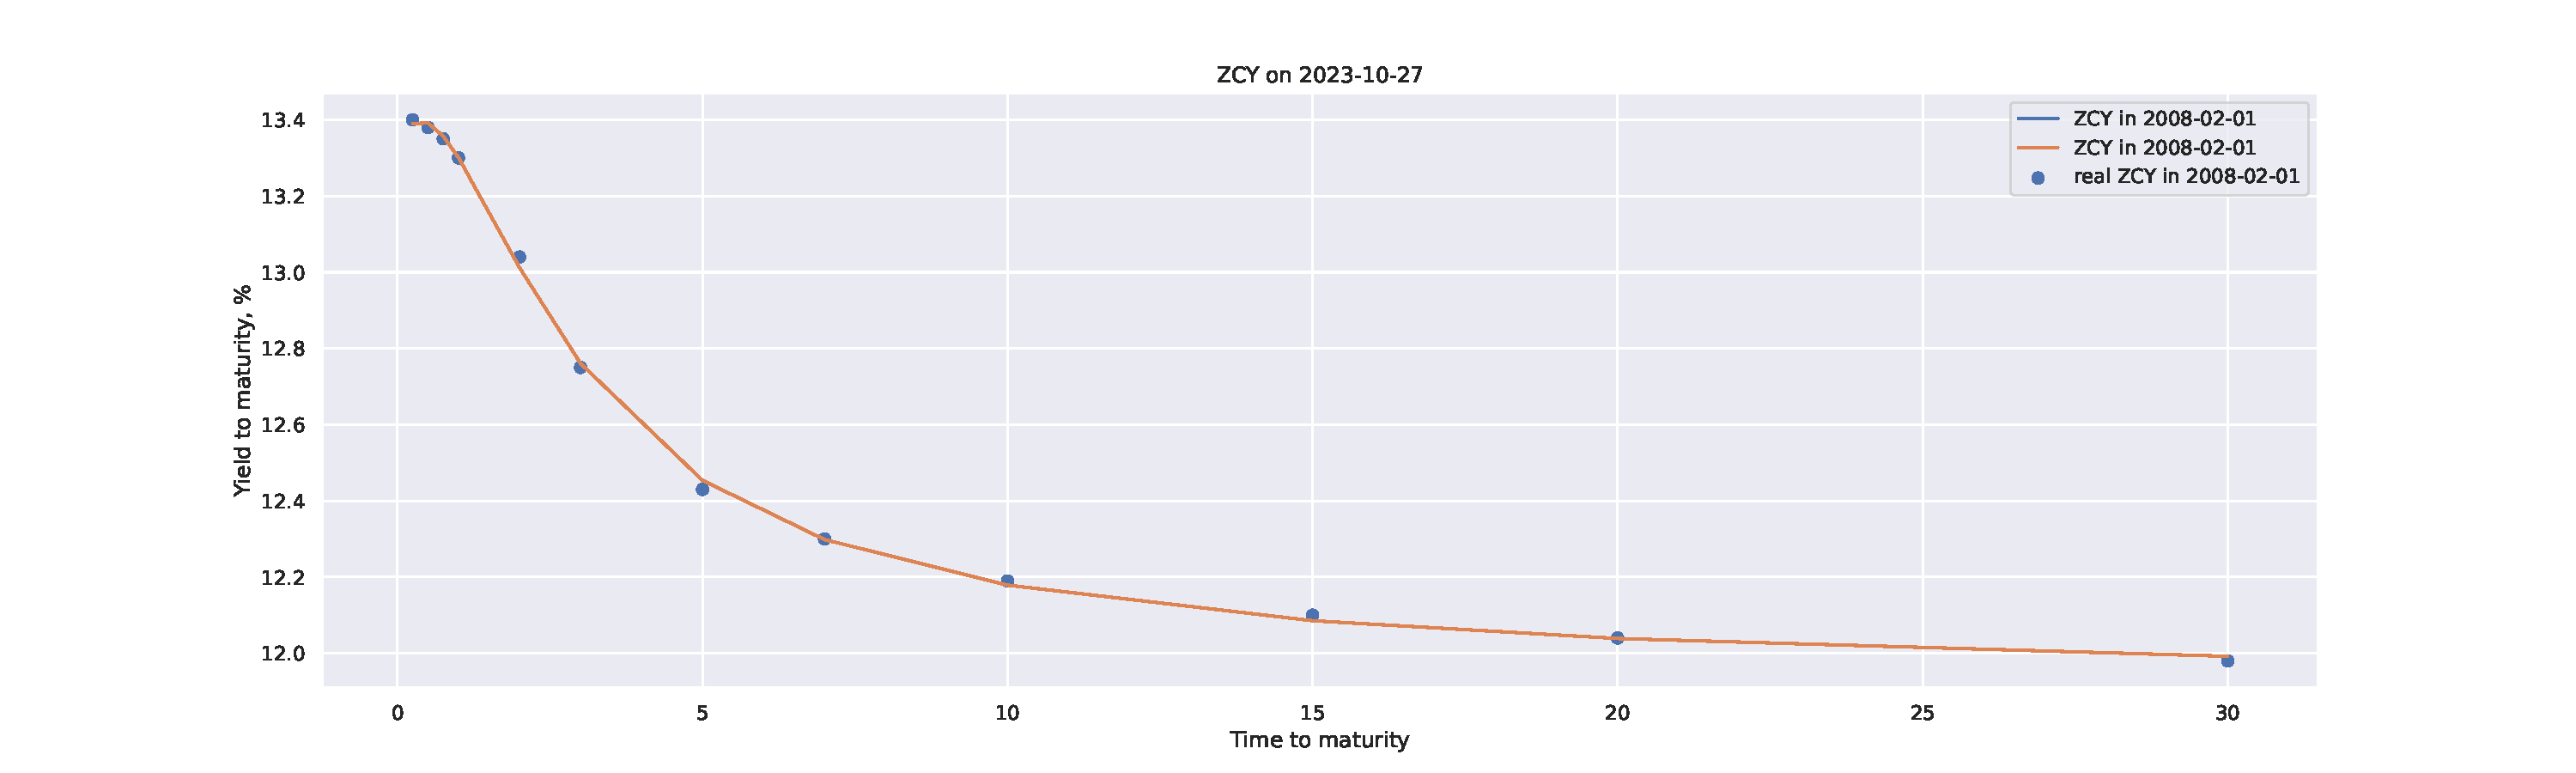
\includegraphics[scale=0.21]{fig/ZCYp.pdf}
        \caption{Yield Curve }
        \label{fig:YTMp}
    \end{figure}
    \begin{equation}\label{eq:NS}
        G(T) = \beta_0 + (\beta_1+\beta_2)\frac{\tau}{T}\left(1-e^{-\frac{T}{\tau}}\right)-\beta_2  e^{-\frac{T}{\tau}},
    \end{equation}
    where $T$ is the time to maturity, $G(T)$ is the yield estimator, 
    and the parameters to be estimated are: $\beta_0$ is the long-run of zero-bond yields, $\beta_1$ is the mid-run of zero-bond yields, 
    $\beta_2$ is the short-run of zero-bond yields.
    
\end{frame}

\begin{frame}{Structural breaks in factors}

    \begin{figure}
        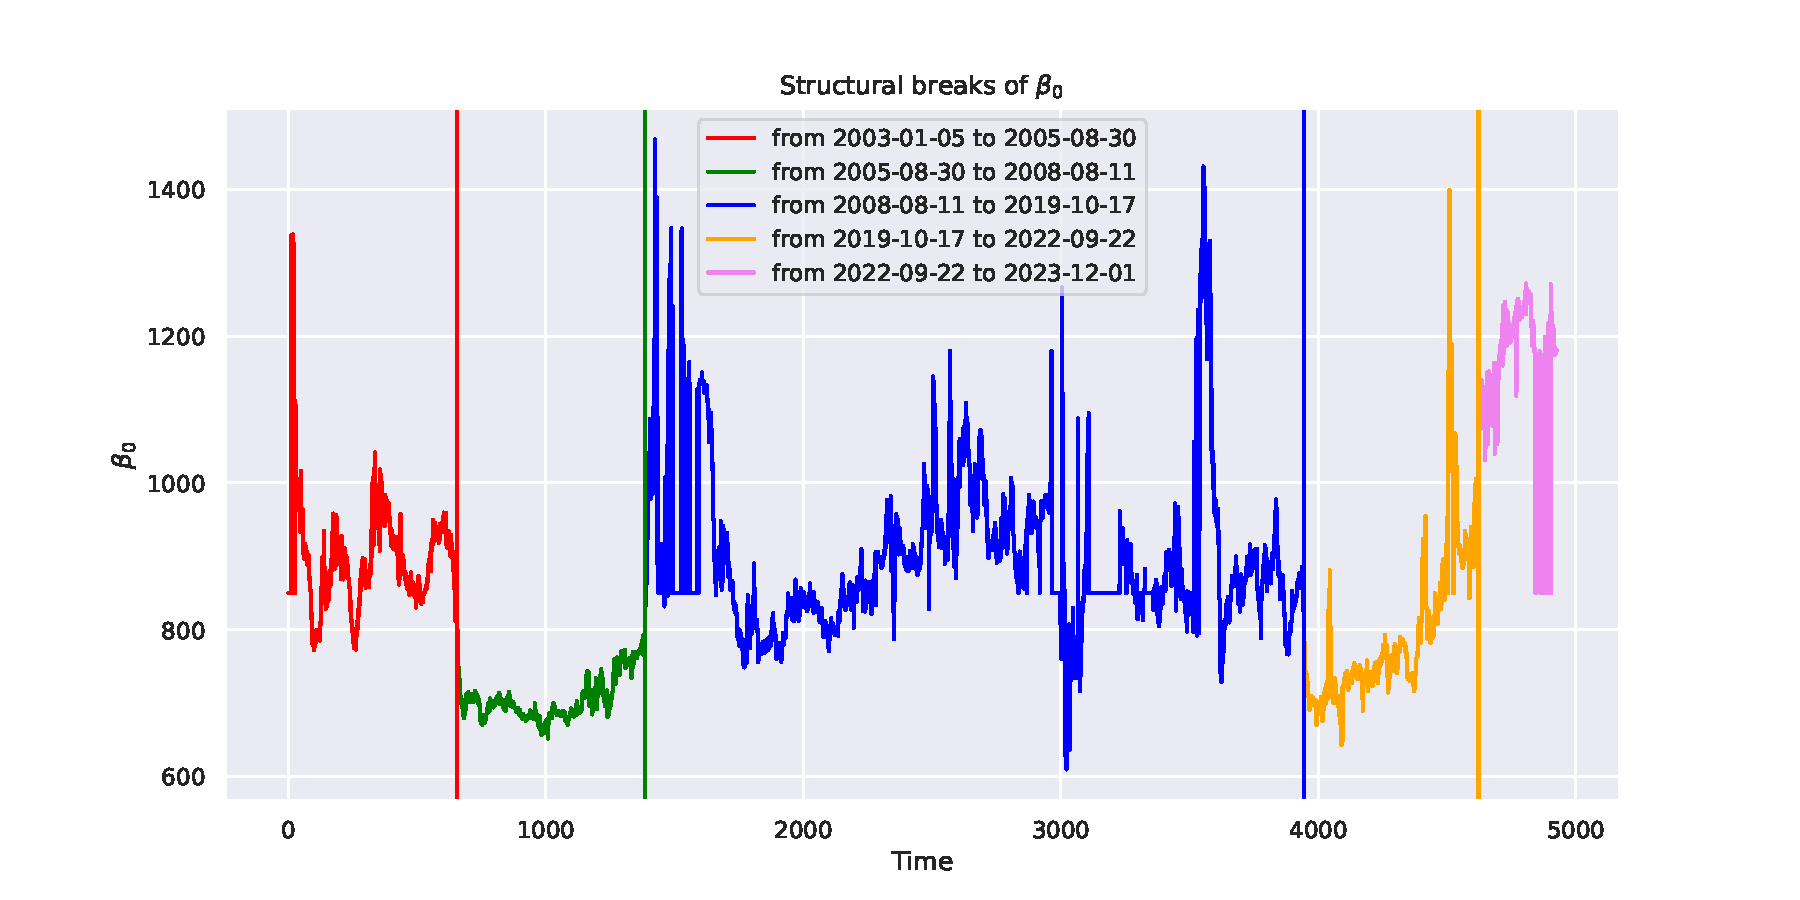
\includegraphics[scale=0.31]{fig/StrBreaks.pdf}
        \caption{Yield Curve }
        \label{fig:StrBreaks}
    \end{figure}
\end{frame}

\begin{frame}{Structural breaks in factors}
    \begin{enumerate}
        \item 2005: The complete stabilization of the Russian economy, the war in Iraq. 
        \item 2008: the Russo-Georgian Conflict and the beginning of the world finanical crisis.
        \item 2018: protests from March 2017 to the end of 2018. Also, it was a 2018 FIFA World Cup.
        \item 2020: COVID-19 pandemic.
        \item 2022: special military operation.
    \end{enumerate}

\end{frame}


    \begin{frame}{Structural breaks}
        \begin{table}[htbp]
            \centering
            \begin{tabular}{|l|l|l|l|l|l|}
            \hline
            Segment            & Factor    & MAPE         & MAE         & RMSE    \\ \hline
            \multirow{ARIMA}{*}{3} & $\beta_0$ & 0.006        & 5.5102      & 6.0729  \\ \cline{2-7} 
                               & $\beta_1$ & 0.3471       & 29.3697     & 32.2907 \\ \cline{2-7} 
                               & $\beta_2$ & 0.5223       & 93.8611     & 95.6724 \\ \cline{2-7} 
                               & $\tau$    & 0.9588       & 1.8988      & 1.987   \\ \hline
            \multirow{VAR}{*}{3} & $\beta_0$ & 0.0139       & 12.8457     & 14.9255     \\ \cline{2-7} 
                               & $\beta_1$ & 0.134        &  12.1766    &  15.9566    \\ \cline{2-7} 
                               & $\beta_2$ &  0.3394      & 60.4861     &  61.5831    \\ \cline{2-7} 
                               & $\tau$    &  0.3582      &  0.68       &  0.7972    \\ \hline
            \end{tabular}
            \caption{NS factors forecasting results for the 3rd segment.}
        \end{table}
    \end{frame}

    \begin{frame}{Nelson-Siegel parametric model}{Model definition}
        The static NS model is defined as follows:
            \begin{equation}\label{eq:NS}
                G(T) = \beta_0 + (\beta_1+\beta_2)\frac{\tau}{T}\left(1-e^{-\frac{T}{\tau}}\right)-\beta_2  e^{-\frac{T}{\tau}},
            \end{equation}
            where $T$ is the time to maturity, $G(T)$ is the yield estimator of the government bonds from the curve basis, 
            and the parameters to be estimated are
            \begin{enumerate}
                \item $\tau$ is the 'typical' time to maturity, 
                \item $\beta_0$ is the long-run of zero-bond yields, 
                \item $\beta_1$ is the mid-run of zero-bond yields, 
                \item $\beta_2$ is the short-run of zero-bond yields.
            \end{enumerate}
    \end{frame}


\end{document}